\section{Realios mašinos projektas}

\subsection{Techninės įrangos komponentai}

\begin{description}
  \item[Procesorius] 
  \item[Naudotojo atmintis]
  \item[Supervizorinė atmintis]
  \item[Duomenų perdavimo kanalai] 
  \item[Įvedimo ir išvedimo įrenginiai.] 
\end{description}

\subsection{Realios mašinos techninės įrangos komponentų išsidėstymo vienas kito atžvilgiu ir tarpusavio sąveikos schema}
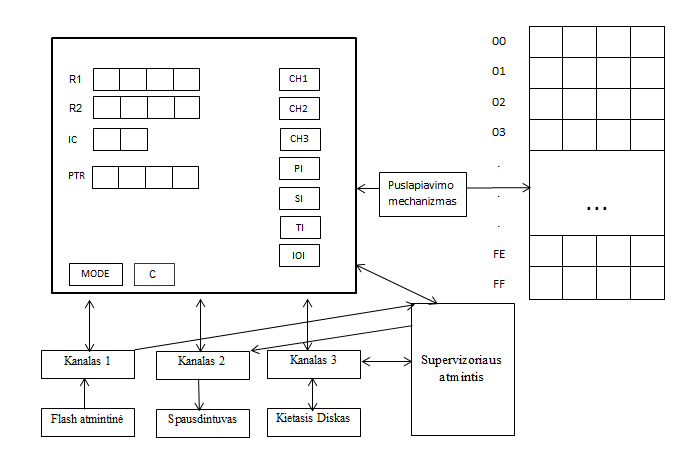
\includegraphics{RM.PNG}
